\documentclass[10pt,a4paper,onecolumn,twoside]{article}
\usepackage[backref=false,bookmarks=false,bookmarksnumbered=false,
            bookmarksopen=false,breaklinks=false,colorlinks=false,
            pdfborder={0 0 1},pdfusetitle,unicode=true]{hyperref}
                                                % for hyperlinks
\usepackage[margin=2.0cm]{geometry}             % to set the margin
\usepackage{fontspec}                           % for fonts
\usepackage{xeCJK}                              % for chinese fonts
\usepackage{float}                              % for figure [H] (here) command
\usepackage{color}                              % for text color
\usepackage{amsmath}                            % for equations
\usepackage{unicode-math}
\usepackage{graphicx}                           % for figures
\usepackage{extarrows}                          % for arrows w/ sub/super-script
\usepackage{tabularx}                           % for tables
\usepackage{multirow}                           % for tables w/ multi-row
\usepackage{authblk}                            % for multiple authors
\usepackage{physics}                            % for easy calculus notations

\numberwithin{equation}{section}                % to add section number to equation numbering
\setlength\parindent{20pt}                      % to set paragraphs' indentation
\setmainfont{Times New Roman}                   % to set English main font
\setmonofont{JetBrainsMonoNL Nerd Font Mono}    % to set English typewriter font
\setsansfont{Helvetica Neue}                    % to set English san-serif font
\setmathfont{STIX Two Math}
\setCJKmainfont{Kaiti TC}[                      % to set Chinese main font
    UprightFont    = * Regular,
    BoldFont       = * Black,
    ItalicFont     = Xingkai TC Light,
    BoldItalicFont = Xingkai TC Bold
]
\setCJKmonofont{NotoSansTC}[                    % to set Chinese typewriter font
    UprightFont    = *-Regular,
    BoldFont       = *-Bold,
    ItalicFont     = *-Thin,
    BoldItalicFont = *-Light
]
\setCJKsansfont{Heiti TC}[                      % to set Chinese san-serif font
    UprightFont    = * Light,
    BoldFont       = * Medium,
    ItalicFont     = Hannotate TC Regular,
    BoldItalicFont = Hannotate TC Bold
]

\AtBeginDocument{
    \renewcommand{\Authfont}{\Large}  % to set author's name font size
    \renewcommand{\Affilfont}{\small} % to set author's affil. font size
    % \renewcommand{\Authsep}{、}       % for authors' names in Chinese
    % \renewcommand{\Authand}{ 和 }
    % \renewcommand{\Authands}{ 和 }

    % \renewcommand{\figurename}{圖}
    % \renewcommand{\tablename}{表}

    \renewcommand{\arraystretch}{1.5}
    \renewcommand{\tabularxcolumn}[1]{m{#1}}
    \setlength{\tabcolsep}{0.1cm}
    \newcolumntype{C}{>{\centering\arraybackslash}X}
    \newcolumntype{R}{>{\raggedleft\arraybackslash}X}
    \newcolumntype{L}{>{\raggedright\arraybackslash}X}
}

\begin{document}

% REMEMBER TO CHANGE DOCUMENT'S PROPERTIES

\title{\huge\textbf{Logic Synthesis and Verification}\\\Huge\textbf{Programming Assignment 1 Report}}
    \author{Yu-Chen Liu}
    \affil{B14901091}
    \date{\today}
\maketitle

% START HERE!
\section{Using ABC}

The \texttt{show} command did not work on my laptop\footnote{It kept throwing me \texttt{sh: gv: command not found} error message. I think it was an environmental issue.},
so I instead outputed as \texttt{.dot} file and rendered it with \texttt{xdot} software externally.
The commands were executed as shown below.

\begin{figure}[H]
    \begin{center}
        \includegraphics[width=0.8\textwidth]{figures/Terminal_Screenshot_1.png}
    \end{center}
    \caption{The screenshot of terminal}
\end{figure}

The results were then rendered.

\begin{figure}[H]
    \begin{center}
        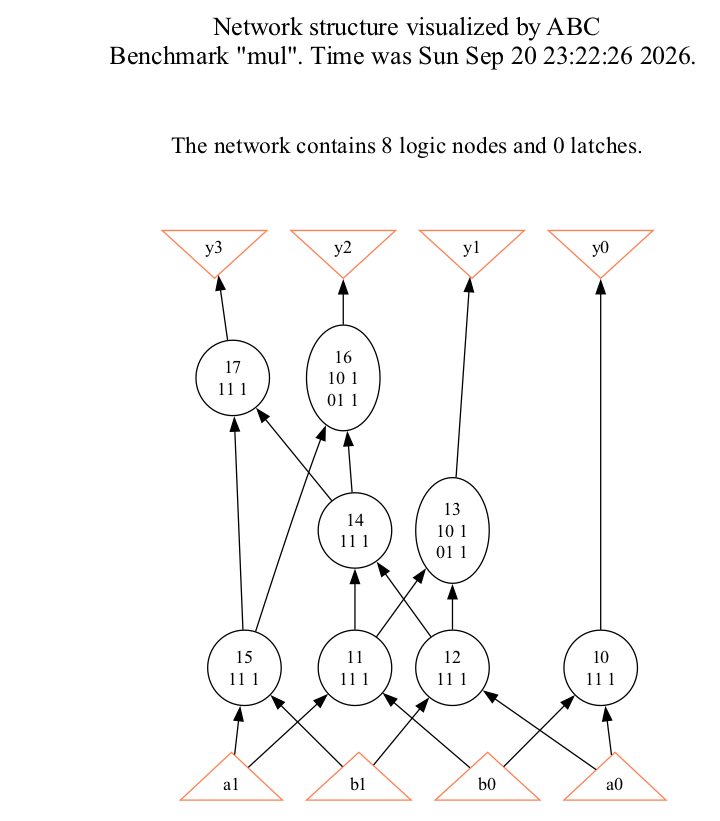
\includegraphics[width=0.3\textwidth]{figures/mul.png}
        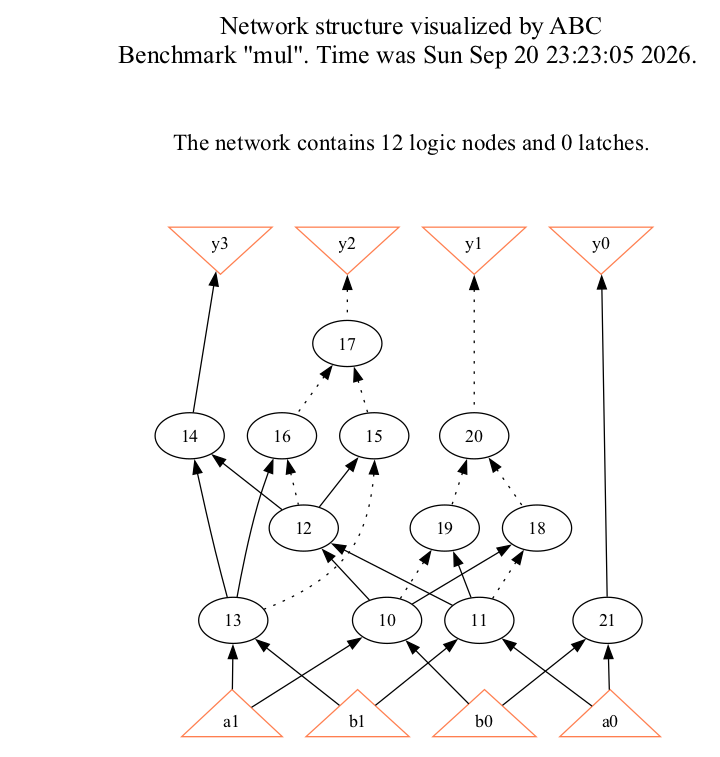
\includegraphics[width=0.3\textwidth]{figures/mul_strash.png}
        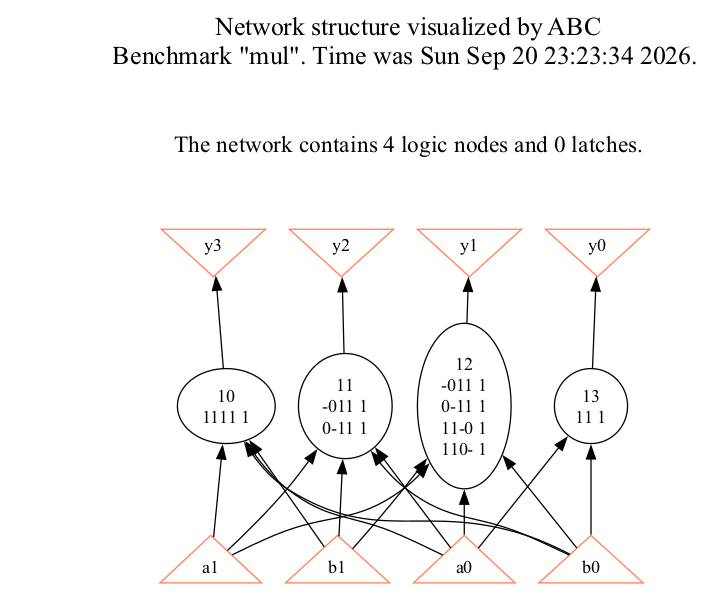
\includegraphics[width=0.3\textwidth]{figures/mul_collapse.png}
    \end{center}
    \caption{The rendered result (left: original, middle: strashed, right: collapsed)}
\end{figure}

\section{ABC Boolean Function Representations}

\subsection{Comparison}

The following shows the executed sequence of command.

\begin{figure}[H]
    \begin{center}
        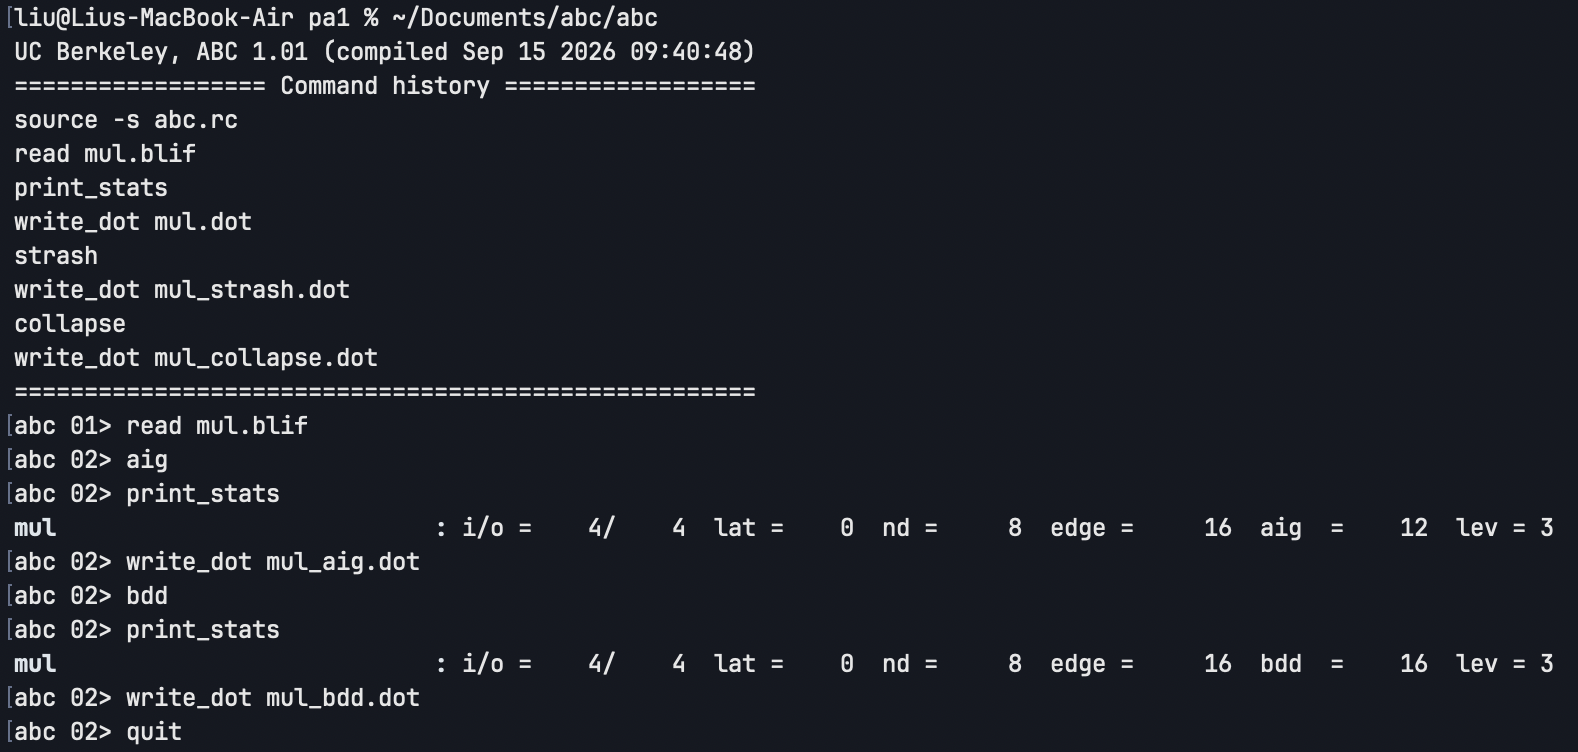
\includegraphics[width=0.8\textwidth]{figures/Terminal_Screenshot_2.png}
    \end{center}
    \caption{The screenshot of terminal}
\end{figure}

The difference can then be compared.

\begin{figure}[H]
    \begin{center}
        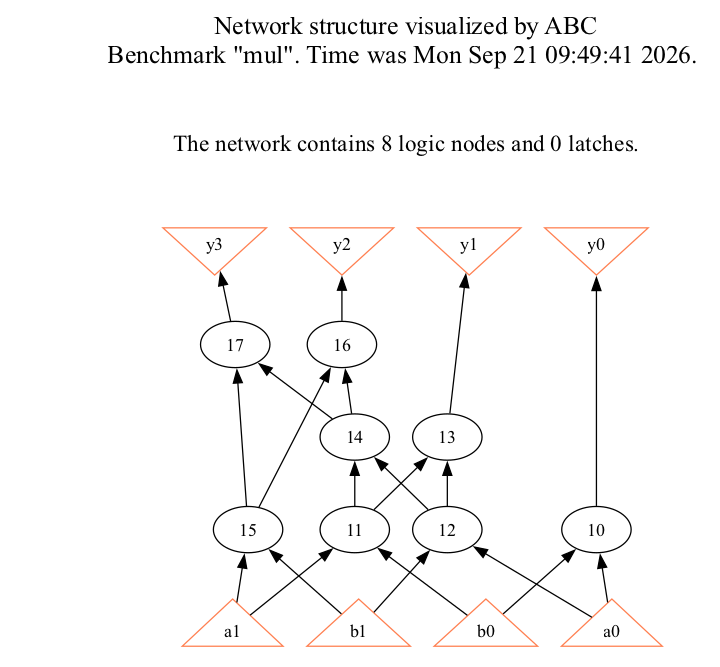
\includegraphics[width=0.45\textwidth]{figures/mul_aig.png}
        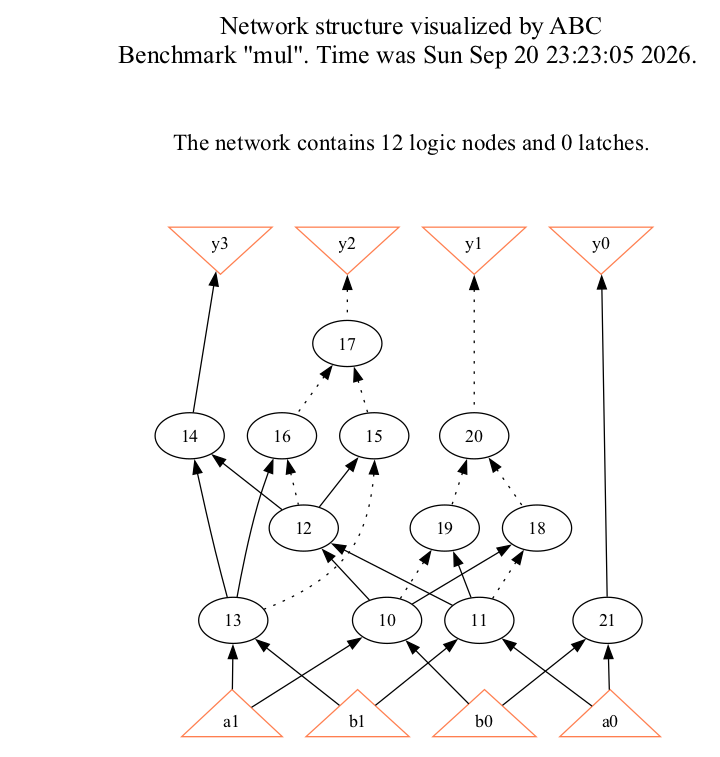
\includegraphics[width=0.45\textwidth]{figures/mul_strash.png}
    \end{center}
    \caption{Multiplier in AIG (left) vs. strashed (right) form}
\end{figure}

The structure in AIG format is the same as the original.
The \texttt{aig} command simply changes the module to aig format in ABC implicitly.
We can see this when \texttt{print\_stats} is executed.
Meanwhile, \texttt{strash} command changes the structure, making each node a two-input single AND-inverter gate.

\begin{figure}[H]
    \begin{center}
        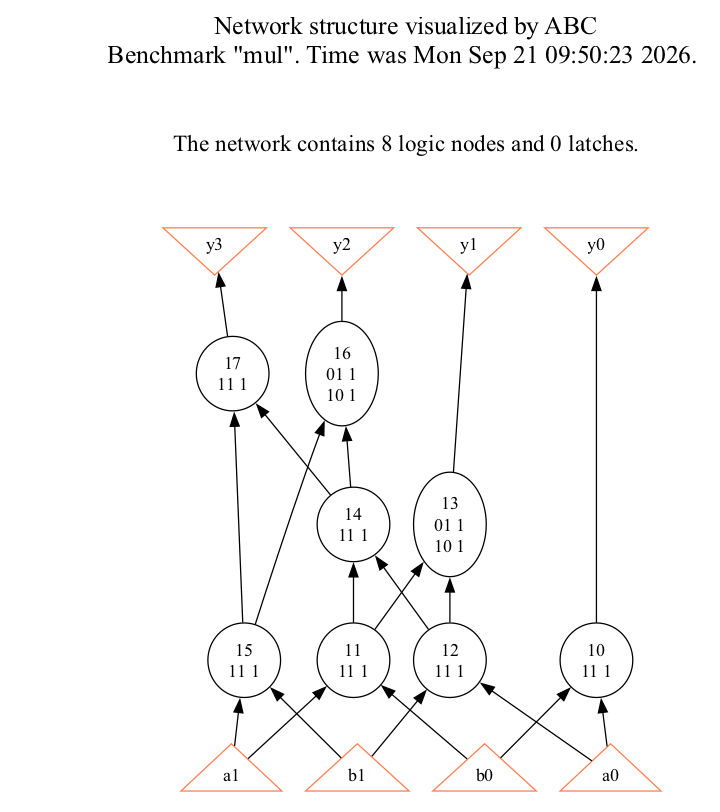
\includegraphics[width=0.45\textwidth]{figures/mul_bdd.png}
        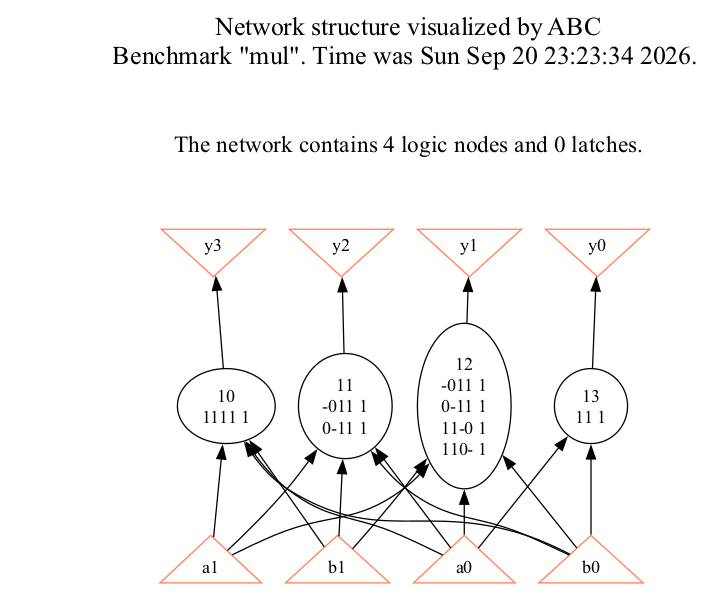
\includegraphics[width=0.45\textwidth]{figures/mul_collapse.png}
    \end{center}
    \caption{Multiplier in BDD (left) vs. collapsed (right) form}
\end{figure}

Similarly, the \texttt{BDD} command only changes the format of each node to binary-decision representation,
without changing the structure.
Whereas, the \texttt{collapse} command flattens the structure into 1-level circuit,
with each node equivalent to a binary-decision tree for each primary output.

\subsection{Command Sequence}

The sequence of command is: \texttt{logic} (convert to a logic network) $\rightarrow$ \texttt{sop} (convert the representation for each node to SOP expression).

\begin{figure}[H]
    \begin{center}
        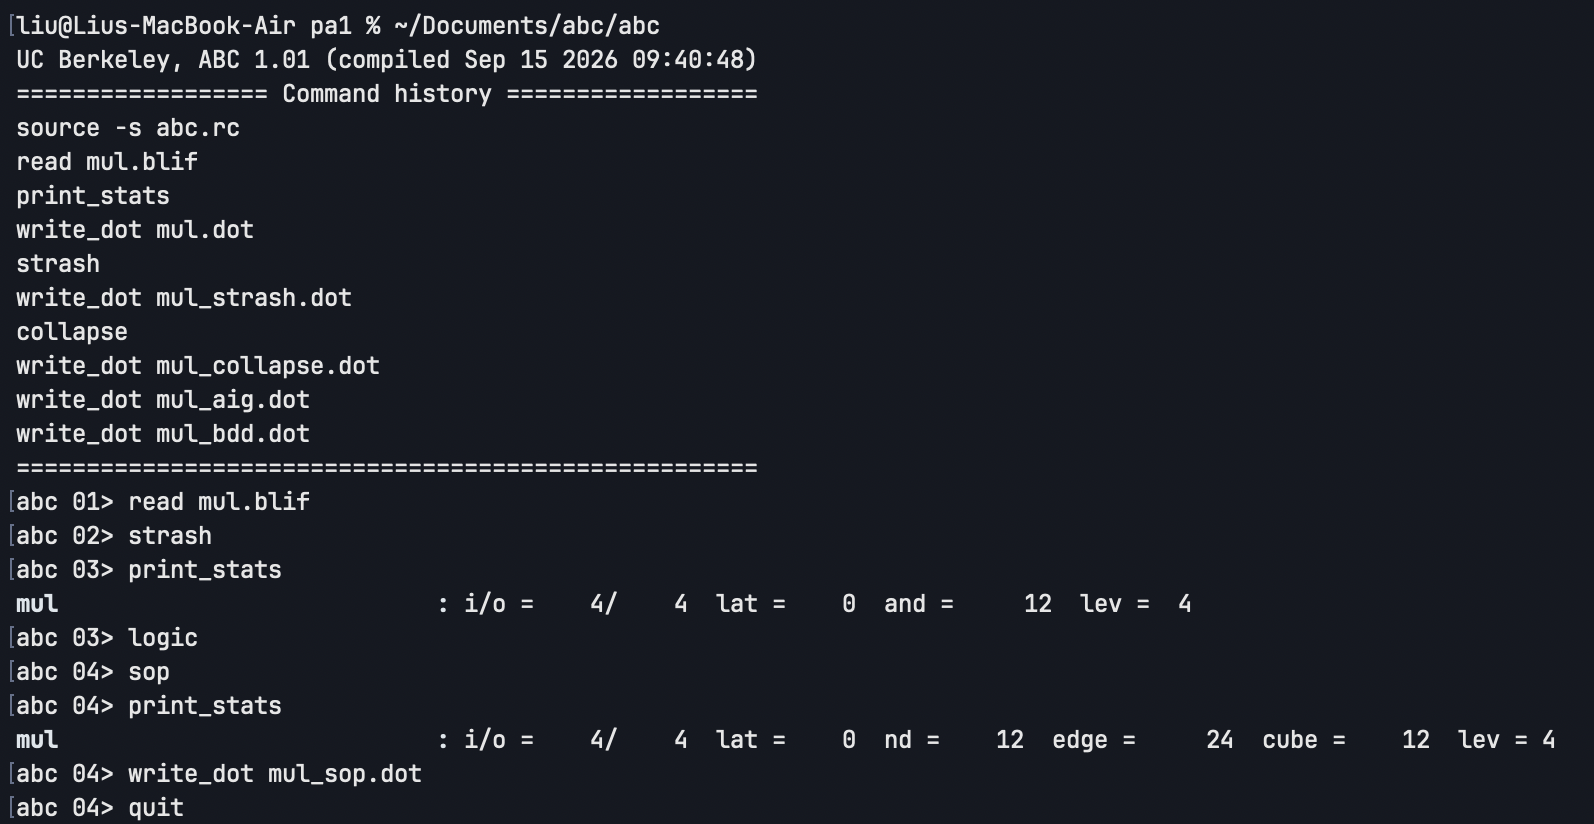
\includegraphics[width=0.8\textwidth]{figures/Terminal_Screenshot_3.png}
    \end{center}
    \caption{The command sequence for transforming a strashed module to a SOP-represented one}
\end{figure}

The result is shown below.

\begin{figure}[H]
    \begin{center}
        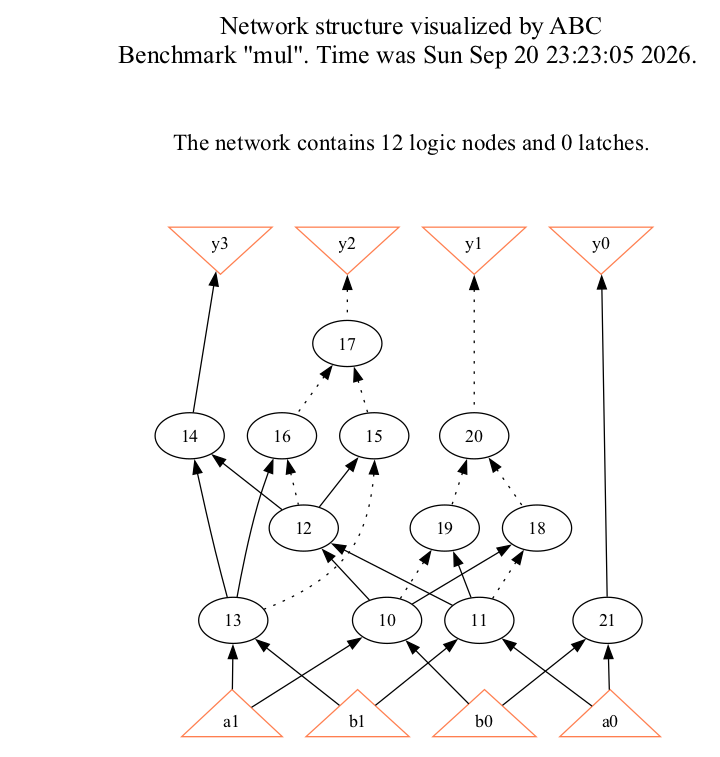
\includegraphics[width=0.45\textwidth]{figures/mul_strash.png}
        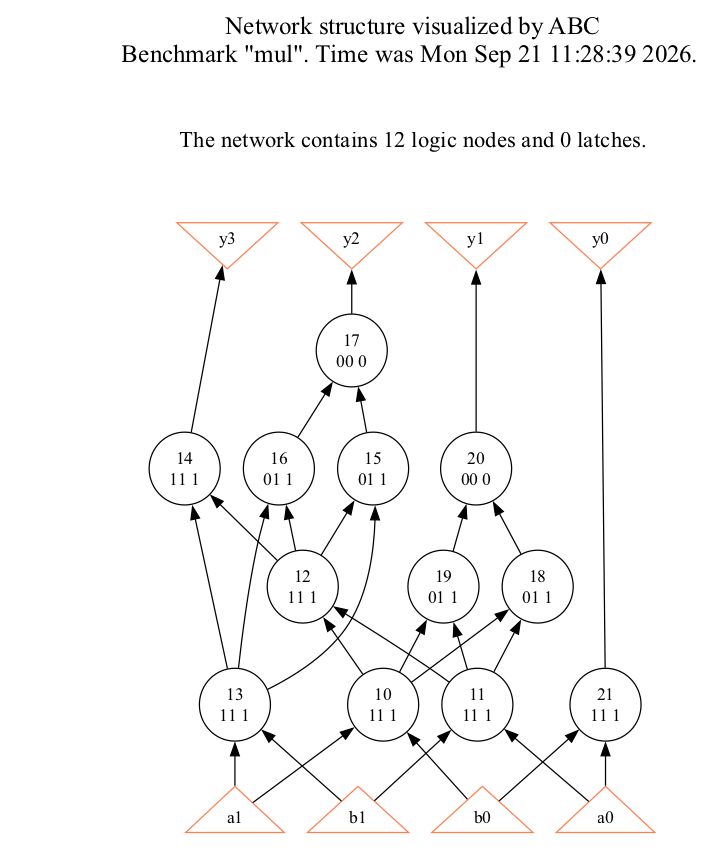
\includegraphics[width=0.45\textwidth]{figures/mul_sop.png}
    \end{center}
    \caption{Before (left) and after (right) the transformation}
\end{figure}

We can see that each node is represented by a SOP expression with single product term.
The output of each node is then determined to be complemented or not for inputs of next nodes.

\end{document}
